\byline{{\textbf{\Large\sffamily Bonsai Events:}}\\
{\textbf{\large\sffamily Chichester's Summer Show}}}{David Fishwick}
\label{2025-07-chichester}
\noindent
On Saturday, 19th July, I had the pleasure of attending the Chichester Bonsai Club's Summer Show at the Manner Nursery: a lovely, free\-to\-enter event that never fails to impress.
As always, the garden centre provided the perfect leafy backdrop for a fantastic gathering of bonsai enthusiasts, with several clubs joining in the fun: the \href{https://www.wvca.co.uk}{Solent Bonsai Society}, the \href{https://sussexbonsaigroup.wordpress.com}{Sussex Bonsai Group}, and of course, the hosts, the \href{https://chichesterbonsai.uk}{Chichester and District Bonsai Club}.

\medskip
The show was a real treat for the eyes, with an outstanding display of trees that showcased the skill and dedication of their owners.
Adding to the excitement was the judging, expertly handled by none other than \textbf{Amelia Williams} --- a good friend of our Bonsai Club and a familiar face to readers, having been featured in last month's \textbf{Shared Canopy} section about her being featured on the \href{https://linktr.ee/themeaningoftreespodcast}{\emph{The Meaning of Trees Podcast}}.
It was a joy watching her thoughtfully evaluate each tree, bringing her keen eye and warm enthusiasm to the task.

\medskip
A highlight of the day was seeing our very own \textbf{Liz Panton} take home \textbf{\textit{Best in Show}} with her stunning \textit{Korean hornbeam} --- a truly deserving winner!
Liz, who is both a steering member of the Chichester and District Bonsai Club and an online member of our club, has once again proven her incredible talent and passion for bonsai.
Congratulations, Liz, for bringing pride to both clubs with your beautiful work!

\medskip
For those who couldn't make it, don't worry: I've included a selection of photos capturing some of the standout trees from the event.
From elegant pines to delicate maples, the variety and artistry on display were a testament to the thriving bonsai community in our region.

\medskip
A quick nod to the practical side of things too: \href{https://www.instagram.com/collettebonsai/}{@ColletteBonsai} and a stand seller kept us well stocked with goodies, ensuring no one went home empty\--handed.
All in all, it was a brilliant day: good company, inspiring trees, and that special buzz that comes from sharing a passion for bonsai.

\medskip
Until next time, happy growing!

\medskip
\hfill\textit{David Fishwick}
\closearticle

\end{multicols}

\medskip
\begin{center}
    \begin{minipage}[b]{.31\textwidth}
        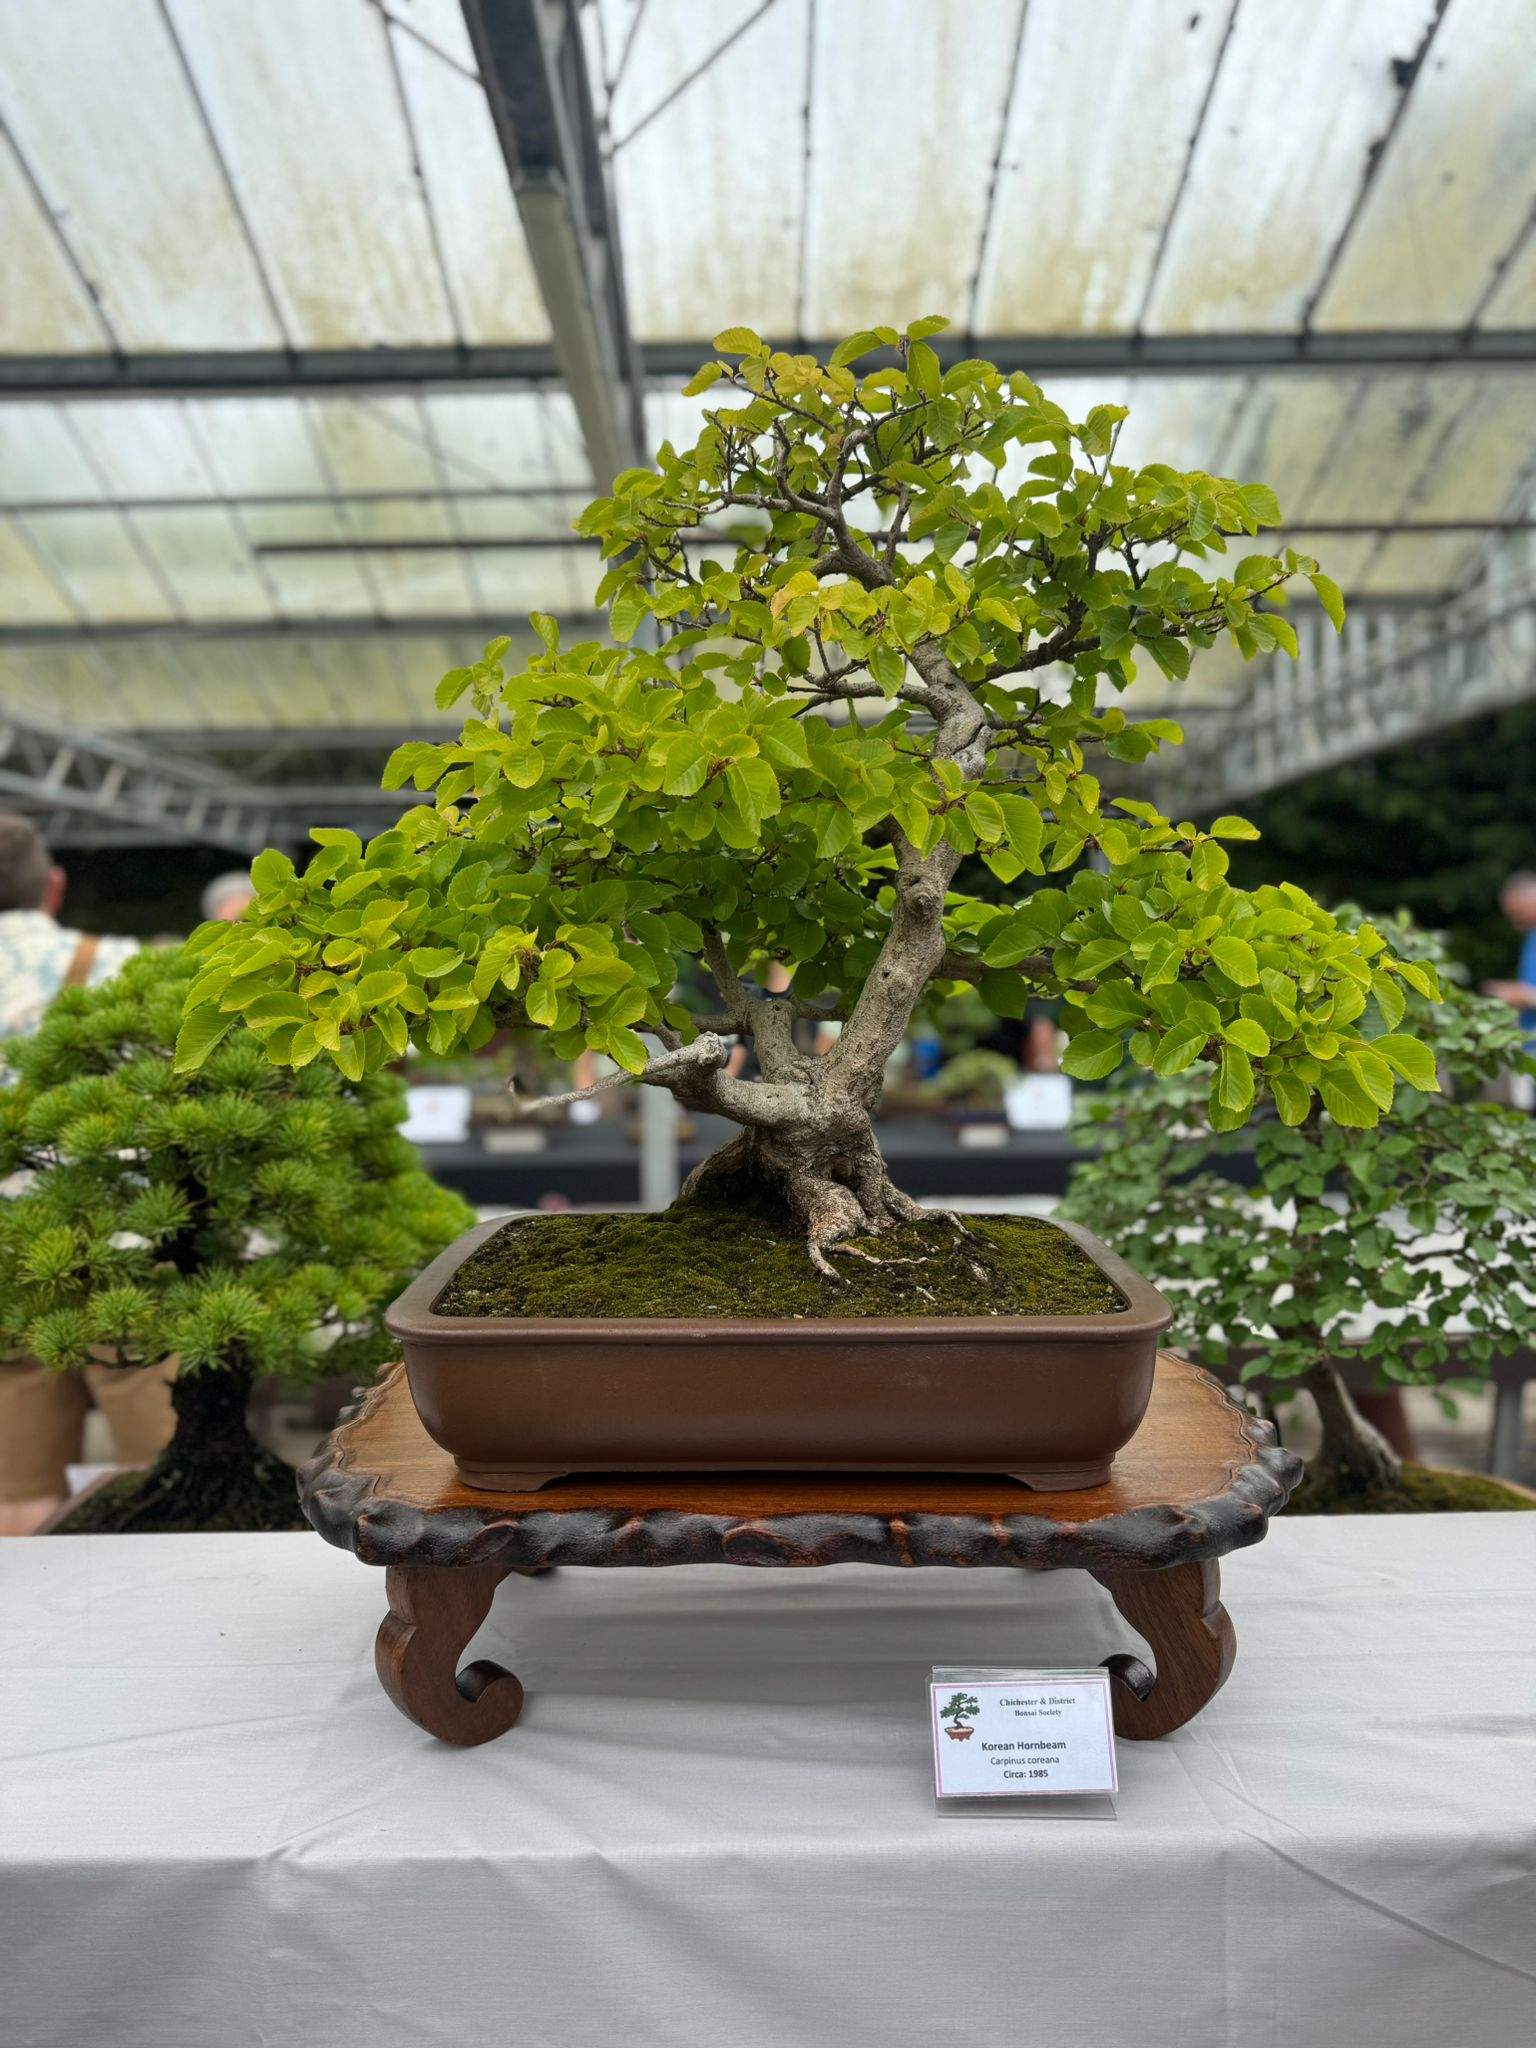
\includegraphics[angle=0,origin=c,width=1.0\textwidth]{2025_07/res/event/chichester_01}
    \end{minipage}\quad
    \begin{minipage}[b]{.31\textwidth}
        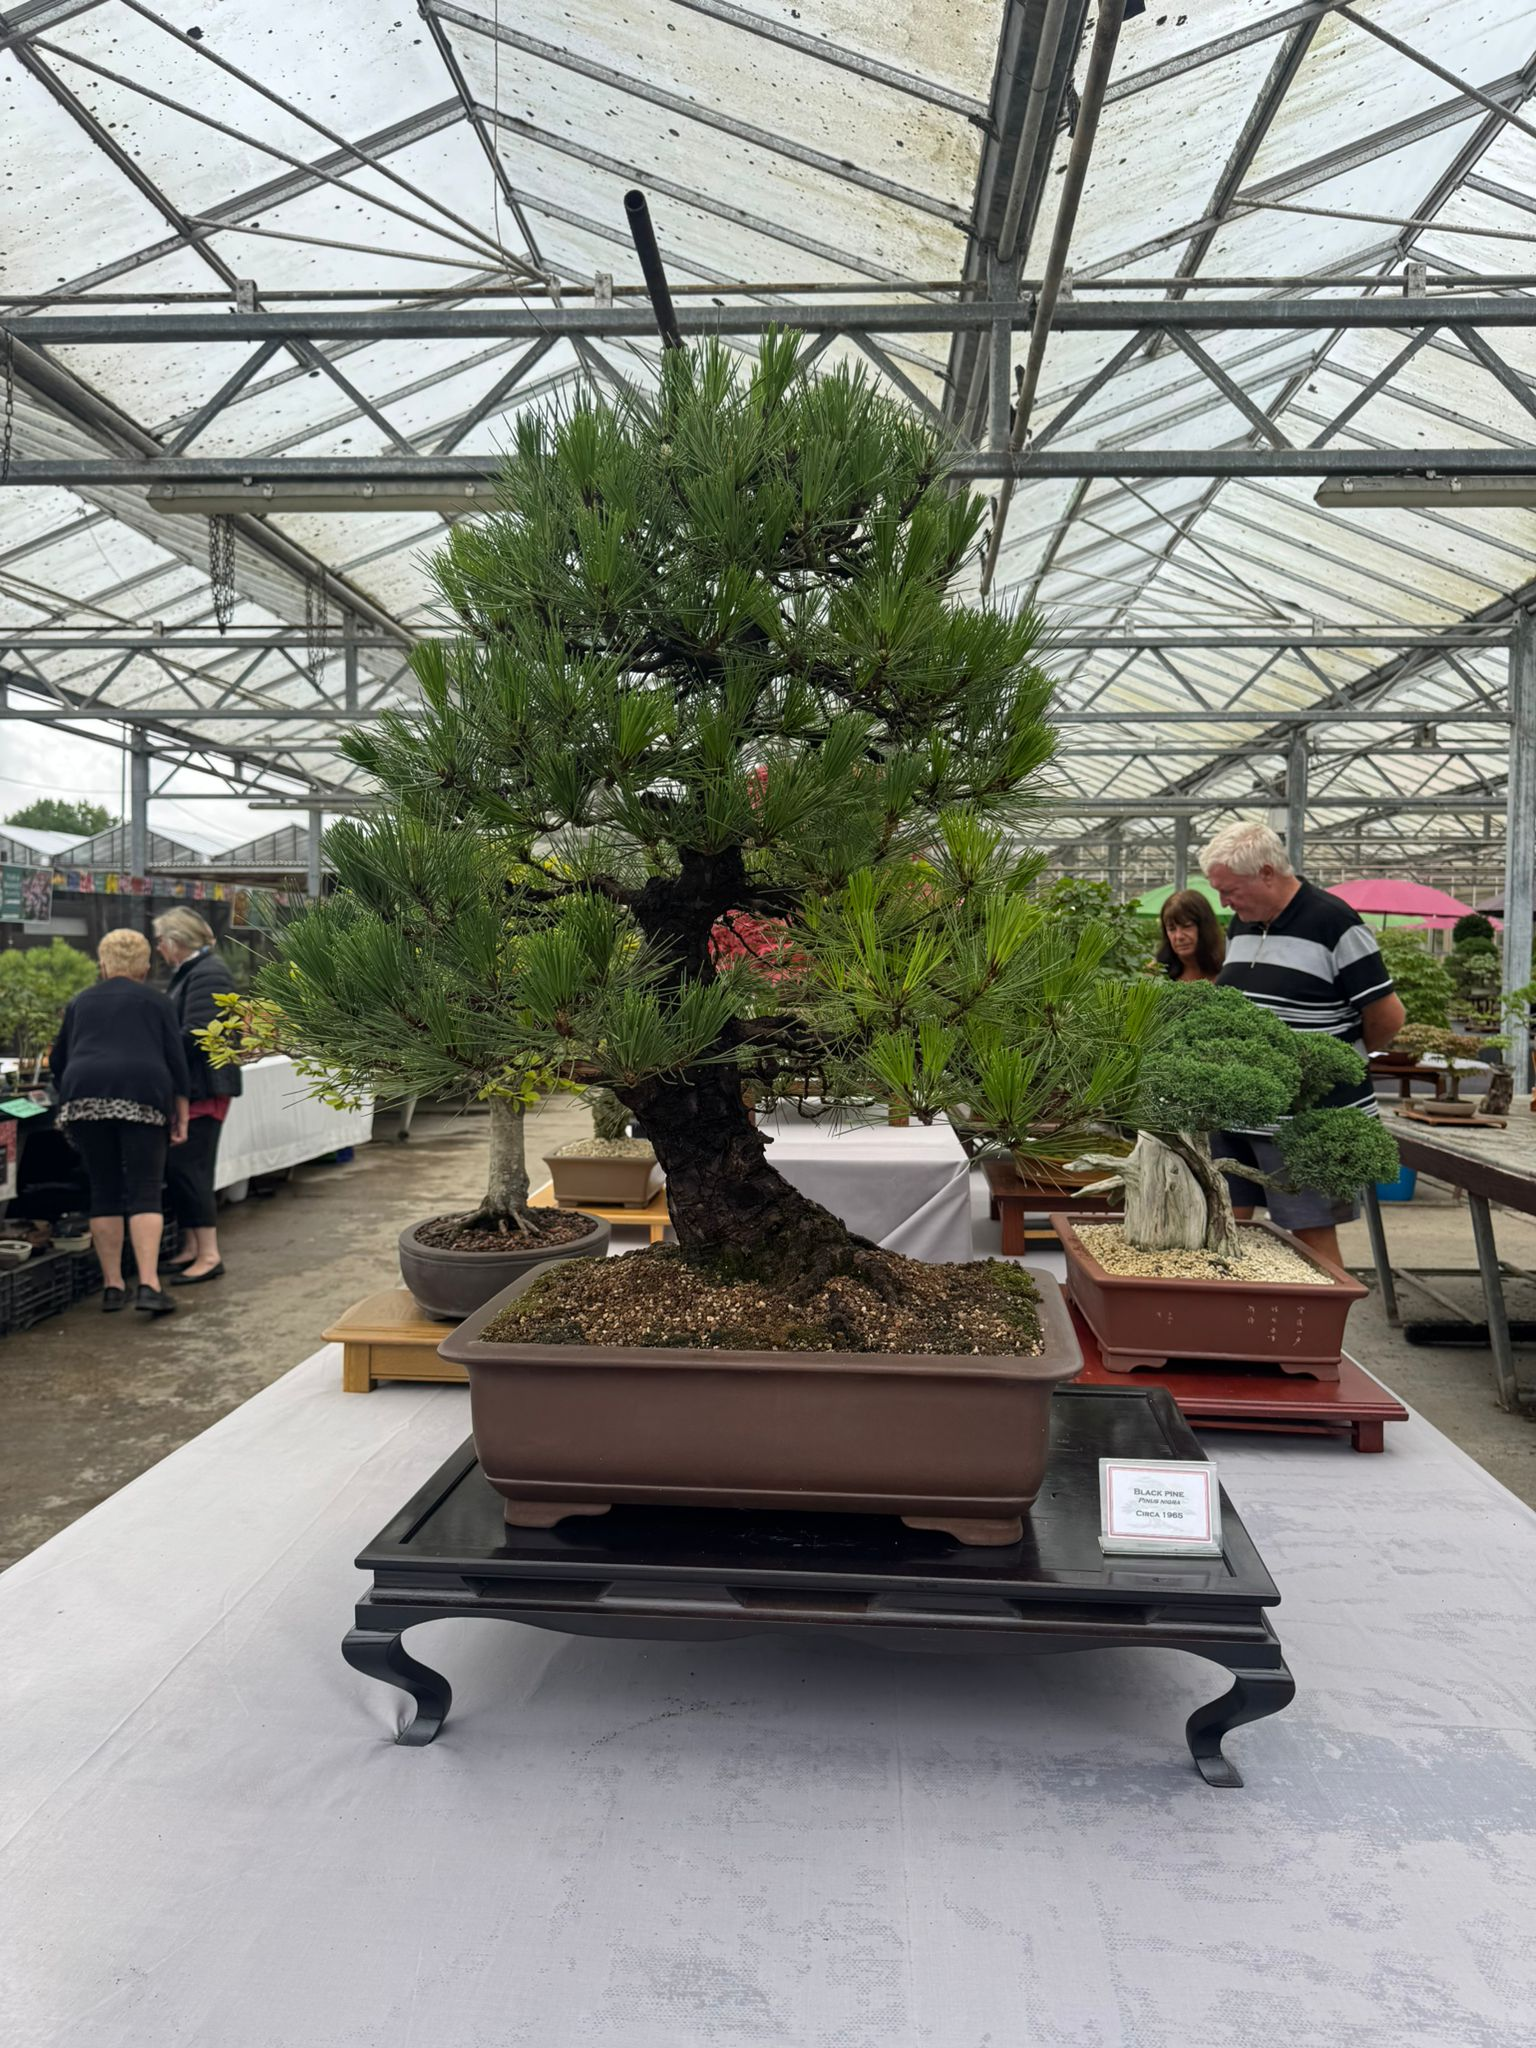
\includegraphics[angle=0,origin=c,width=1.0\textwidth]{2025_07/res/event/chichester_02}
    \end{minipage}\quad
    \begin{minipage}[b]{.31\textwidth}
        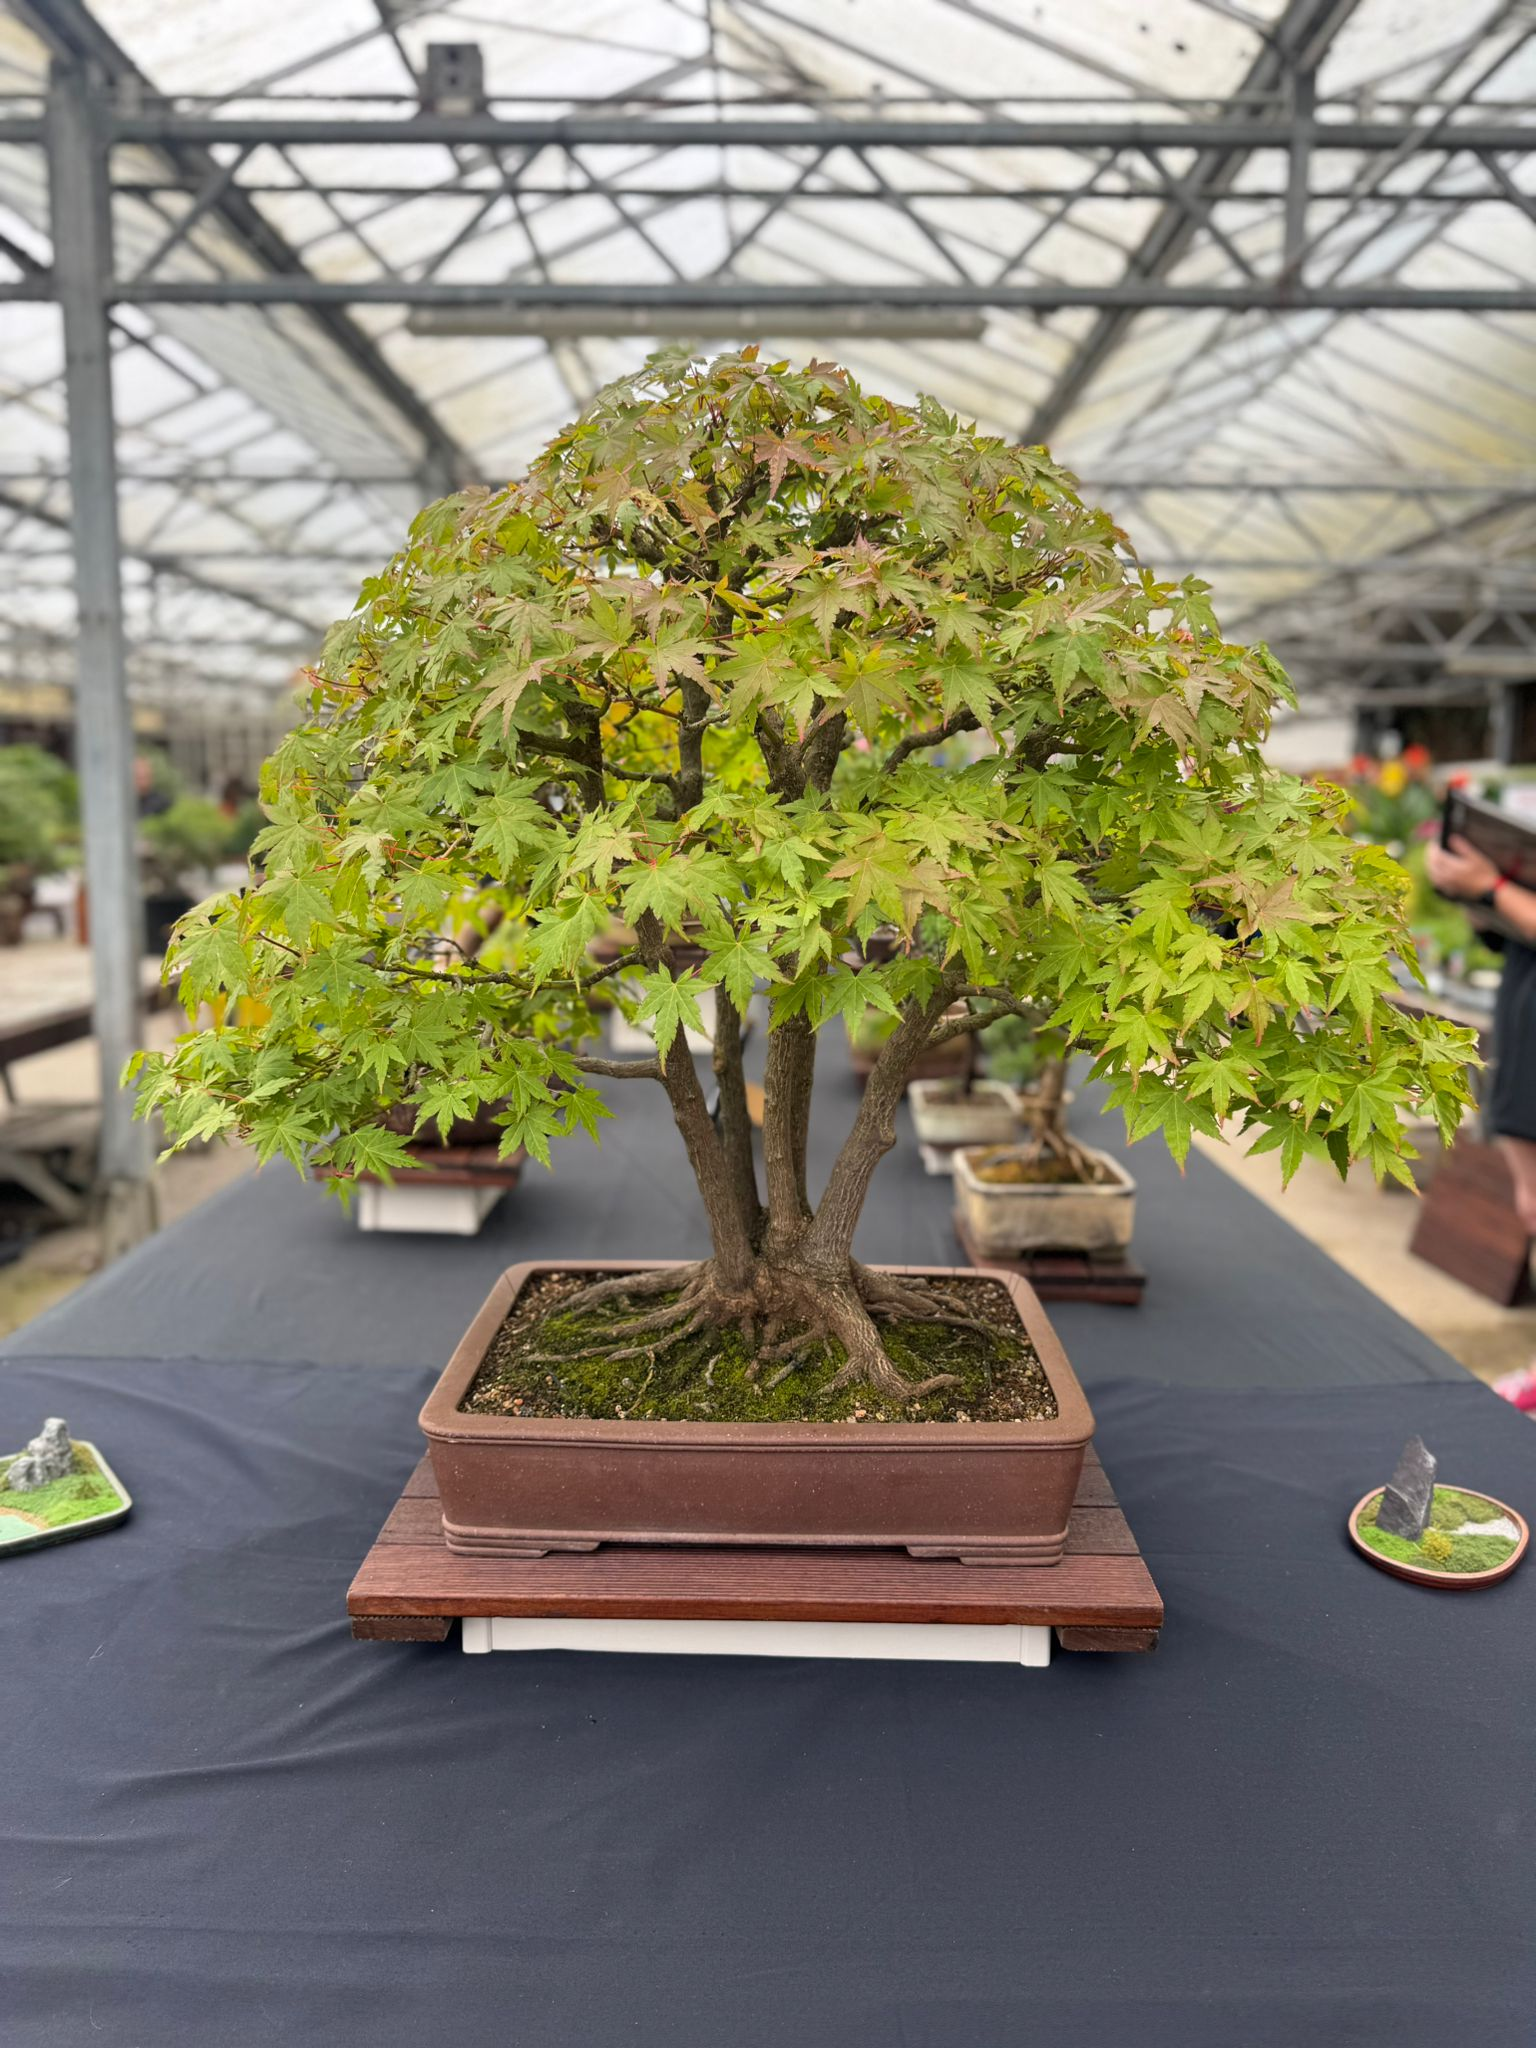
\includegraphics[angle=0,origin=c,width=1.0\textwidth]{2025_07/res/event/chichester_03}
    \end{minipage}
    \medskip

    \begin{minipage}[b]{.31\textwidth}
        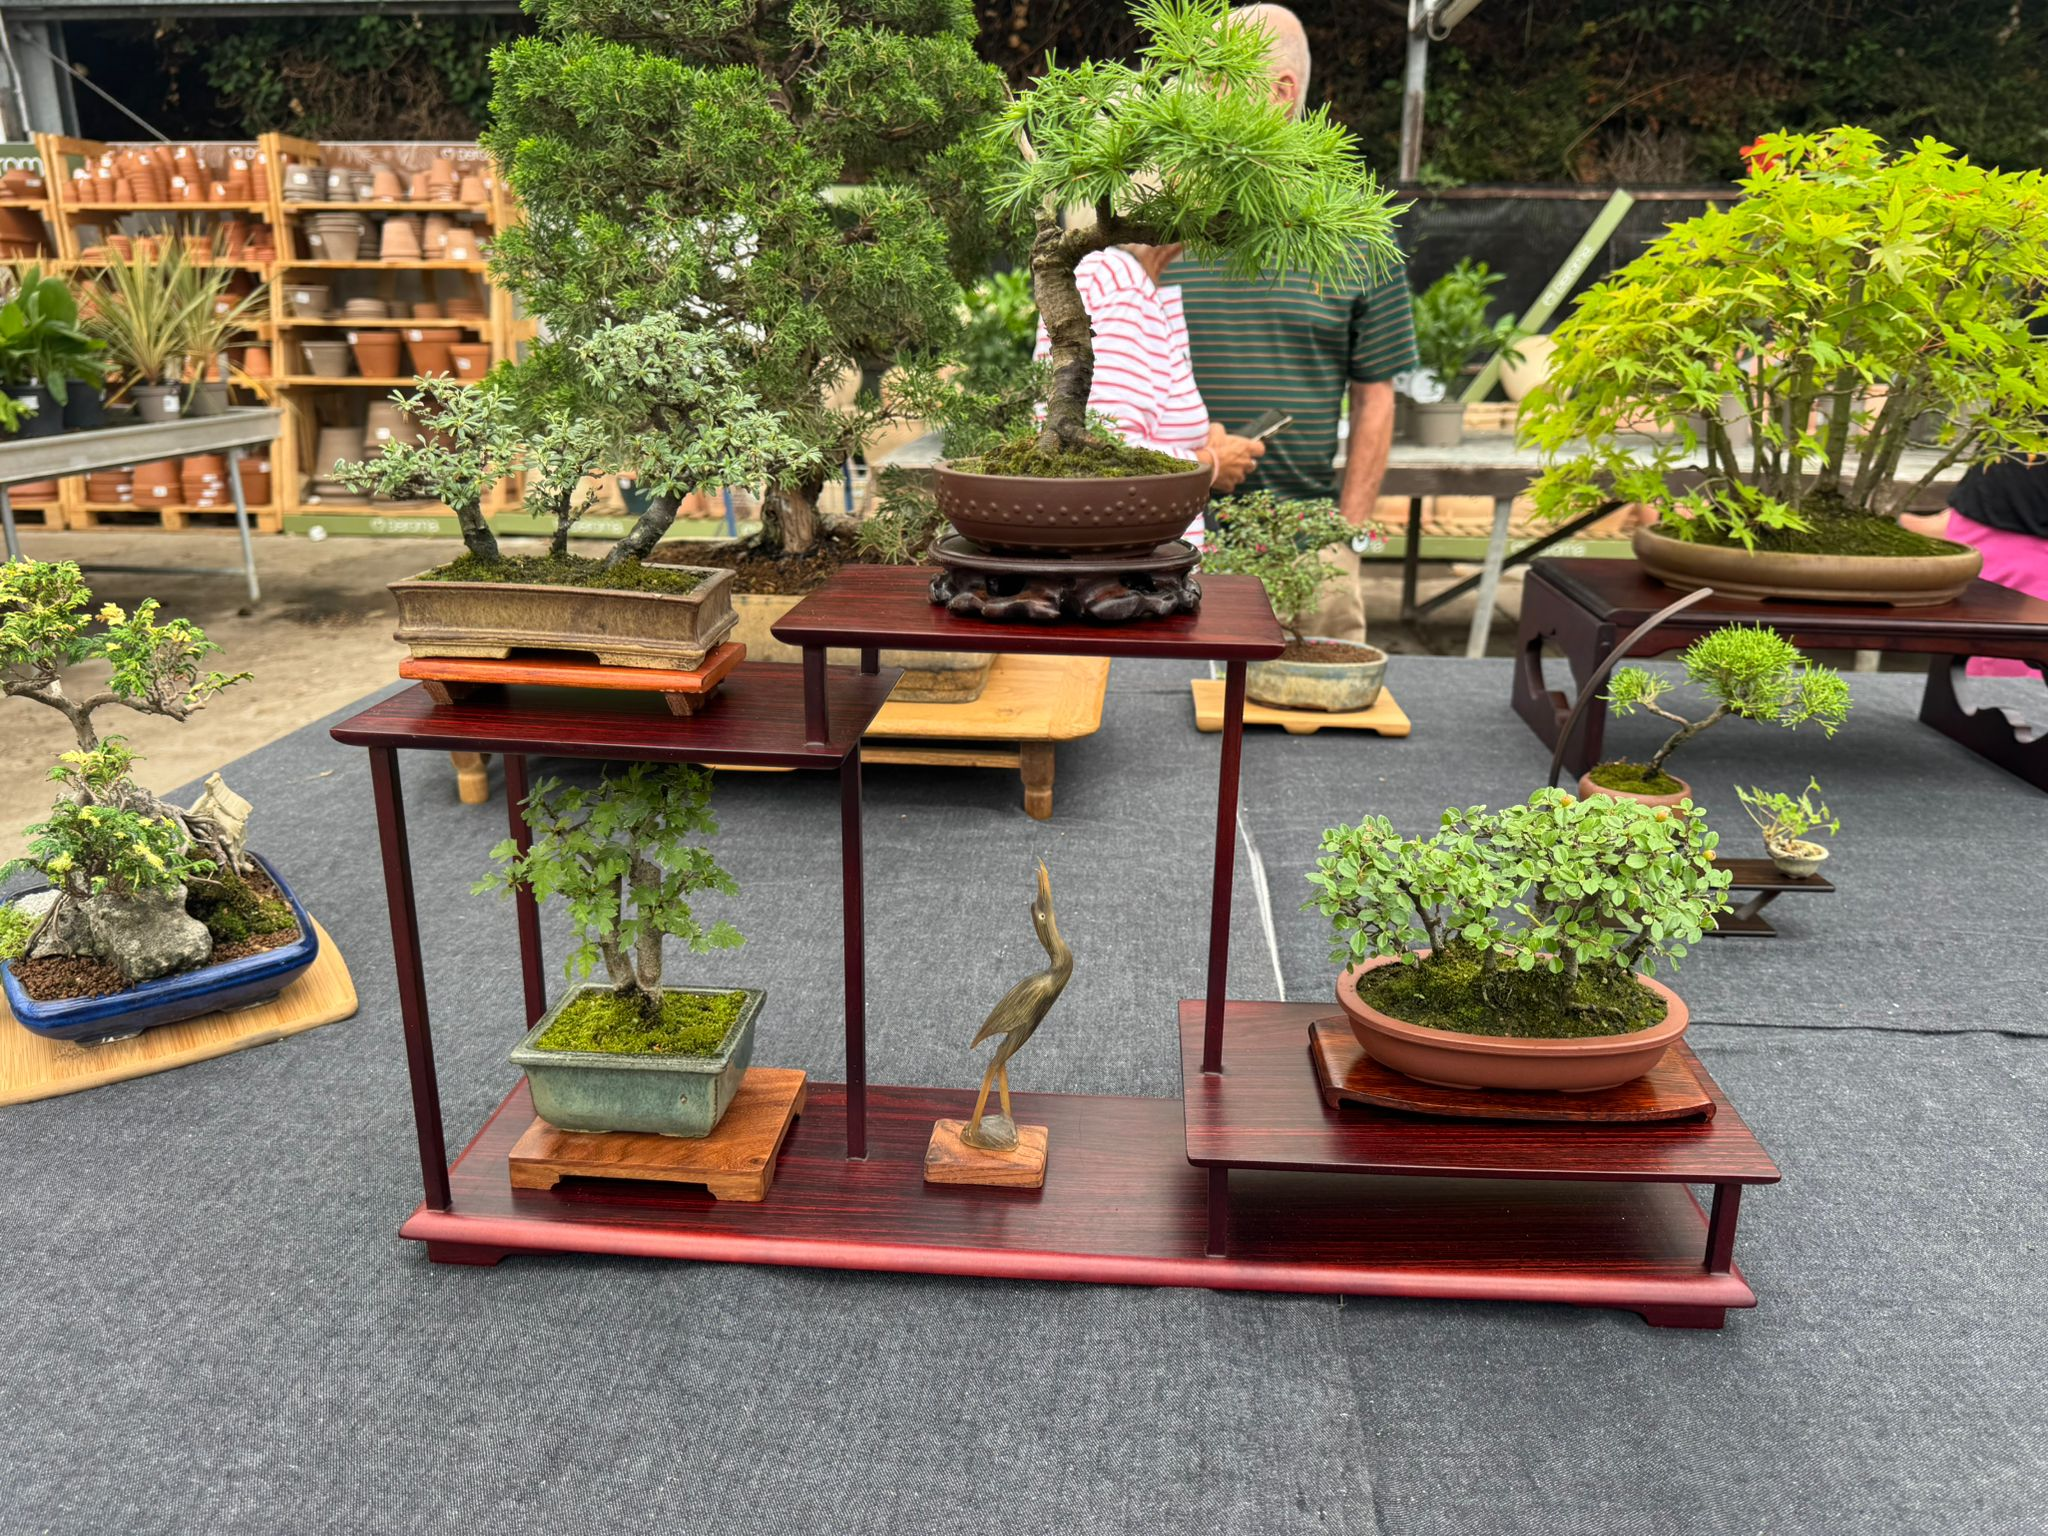
\includegraphics[angle=0,origin=c,width=1.0\textwidth]{2025_07/res/event/chichester_05}
    \end{minipage}\quad
    \begin{minipage}[b]{.31\textwidth}
        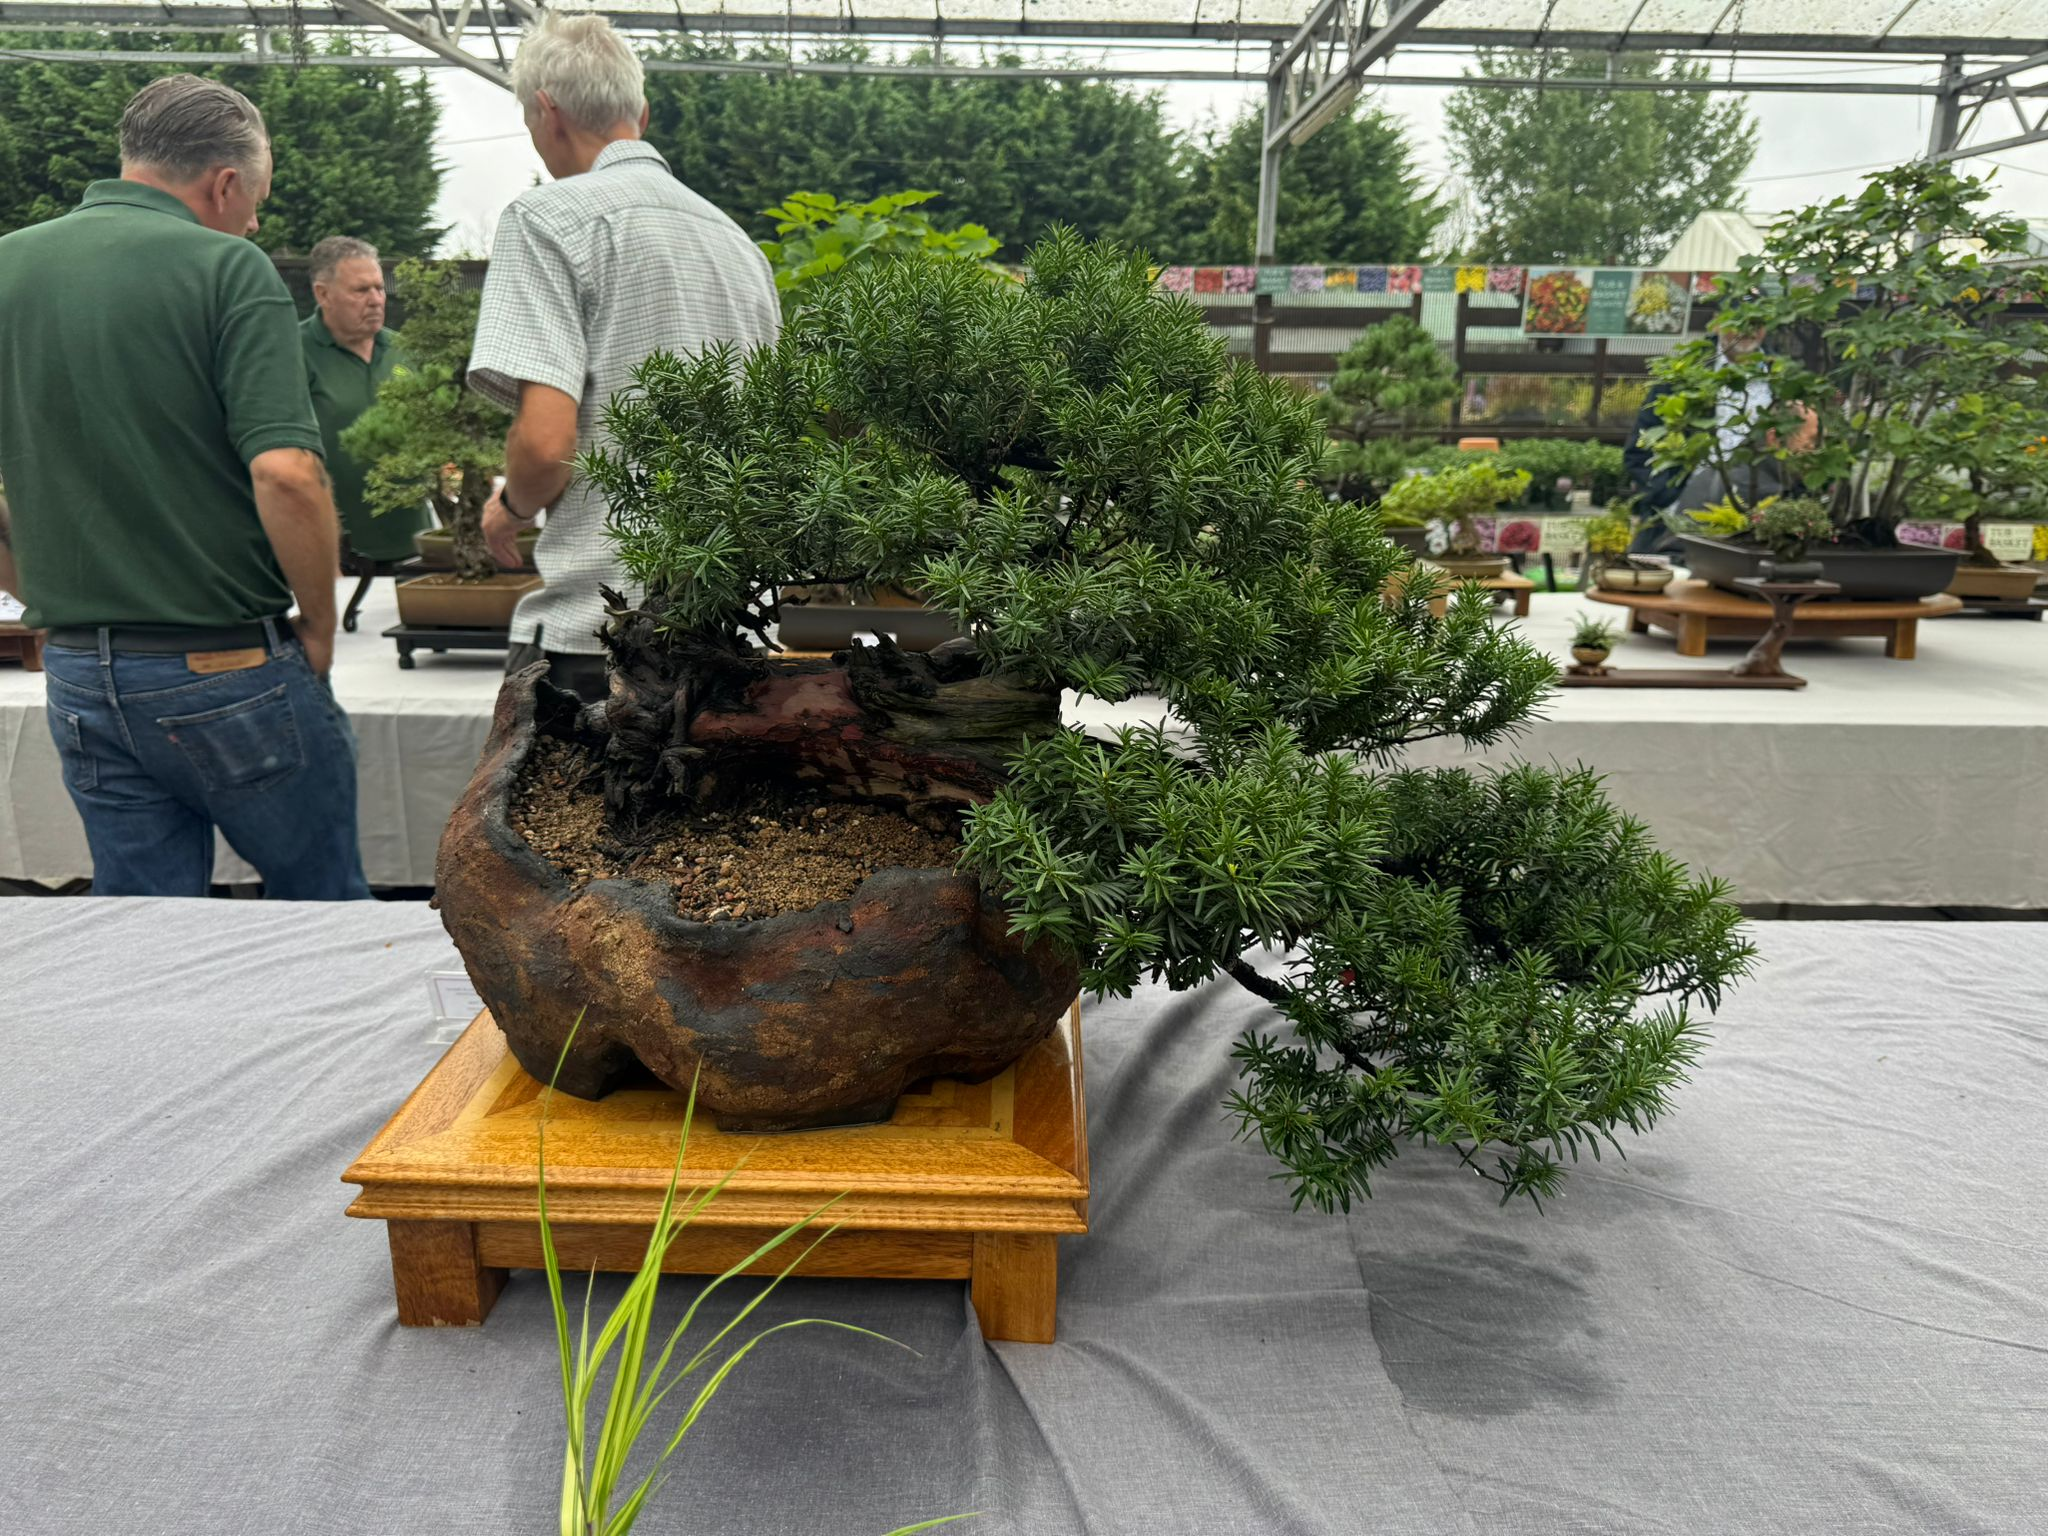
\includegraphics[angle=0,origin=c,width=1.0\textwidth]{2025_07/res/event/chichester_06}
    \end{minipage}\quad
    \begin{minipage}[b]{.31\textwidth}
        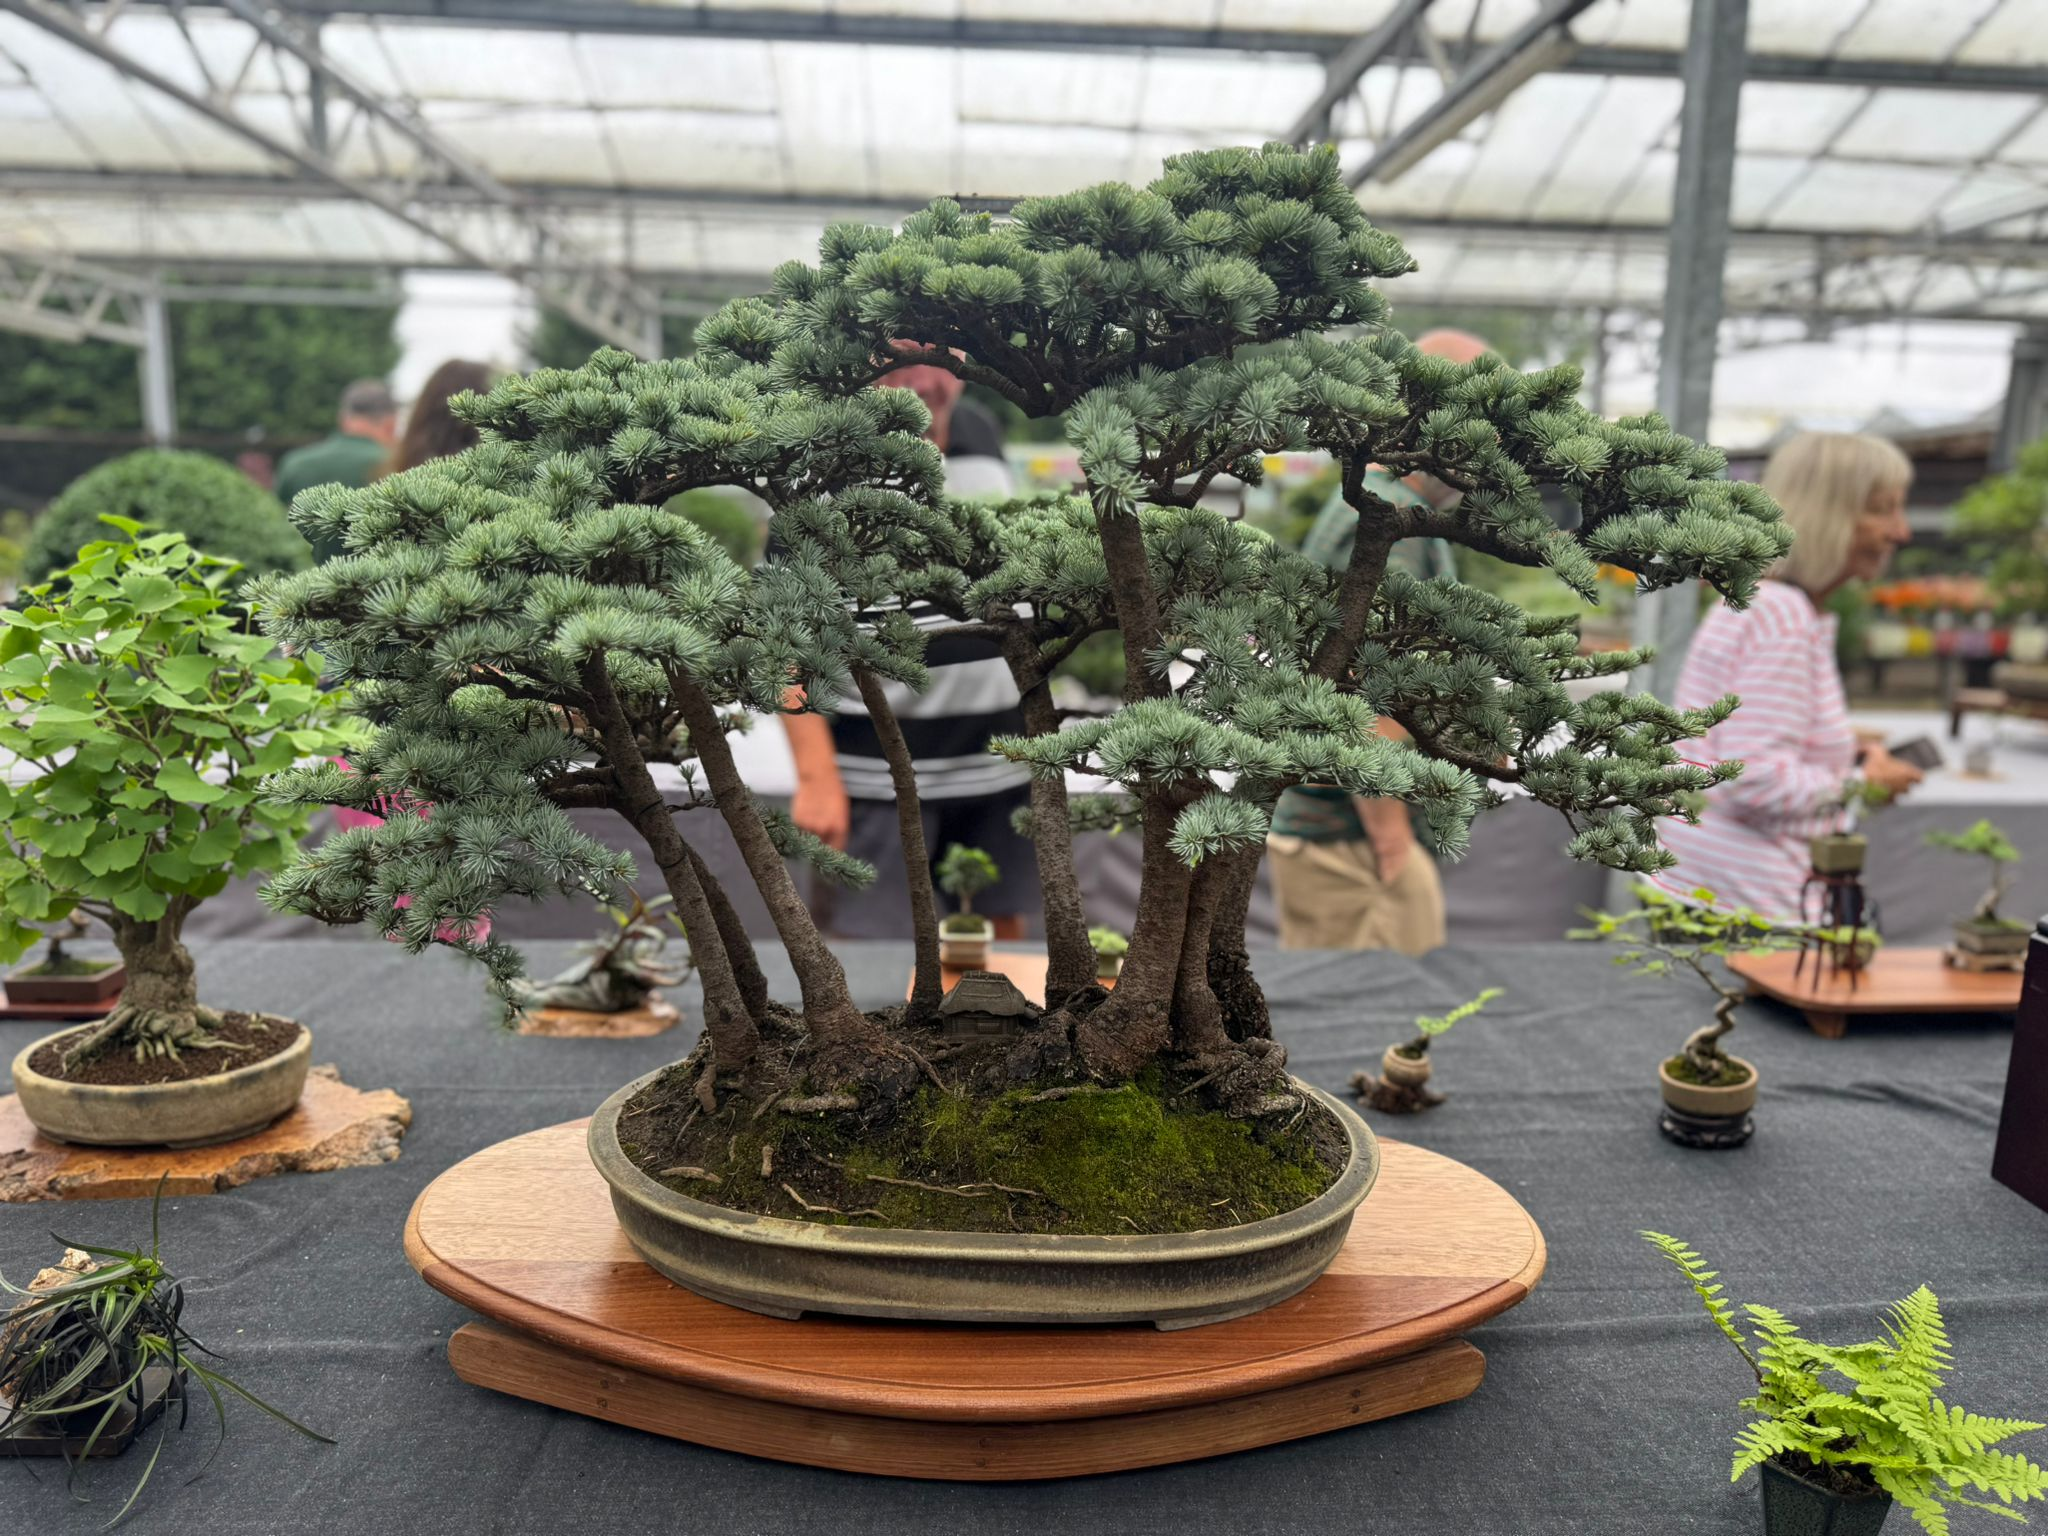
\includegraphics[angle=0,origin=c,width=1.0\textwidth]{2025_07/res/event/chichester_07}
    \end{minipage}
\end{center}
\clearpage

\begin{multicols}{2}
